\chapter{General Discussion}\thumbforchapter
\newpage

\section{The scientific dogma of the phylotypic stage}

\begin{shadequote}[c]{George Box}
All models are wrong, but some are useful.
\end{shadequote}

While historically, the phylotypic stage has predominantly been examined and described through qualitative methods, the 21\textsuperscript{st} century started a paradigm shift towards a more quantitative and data-driven approach to understanding this phenomenon\cite{Chan2021}. The first notable quantitative investigation into the phylotypic stage was done by Bininda-Emonds \textit{et al.}, where they calculated temporal conservation as the order in which morphological embryonic features appear in vertebrates\cite{OlafRP2003}. However, it wasn't until the early 2010s that the field truly embraced quantitative methodologies with the simultaneous publication of two groundbreaking studies in Nature\cite{Kalinka2010, DomazetLoso2010}. In these works, Domazet-Lošo \textit{et al.} investigated the average developmental age of transcripts in \textit{D. rerio} and \textit{D. melanogaster}, whilst at the same time, Kalinka \textit{et al.} explored the temporal transcriptome similarities across different \textit{Drosophila} species. These molecular studies opened a new line of research to the quantitative basis of the phylotypic stage. The quantitative support for the phylotypic stage appeared stronger and stronger with each new study. So strong, that we quickly forgot all the nonconforming studies.

The Transcriptome Age Index (TAI), as introduced by Domazet-Lošo \textit{et al.}, is a metric of the average evolutionary age of transcripts over time\cite{DomazetLoso2010}. Evolutionary age is determined as the number of taxonomic branches to which a gene can be traced back. The central idea of the TAI is that temporal changes in gene expression provide insights into the degree of conservation during development. However, a re-analysis conducted by Piasecka \textit{et al.} raised some critical points about the methodology\cite{Piasecka2013}. Their investigation revealed that the TAI is heavily influenced by a relatively small subset of genes due to major differences in transcript levels per gene (transcriptomic data is notoriously heteroscedastic). Log transforming the data, which is a standard processing step for this type of data, completely invalidates the results of the original study. One might expect such a dependency on data transformation to cast doubts on the method's reliability. Surprisingly, the opposite appears to be true. The original study introducing the TAI has been cited 88 times between 2010 and 2013, and 359 citations since Piasecka \textit{et al.}'s publication (covering the years 2014-2023). As it turns out, you can now analyze the data with and without transformation, and keep the results that reinforce your preferred hypothesis. A notable example of this is found in Wu \textit{et al.}'s study on Spiralian development\cite{Wu2019}. In their analysis of untransformed data for \textit{Crassostrea gigas}, \textit{Haliotis discus hannai}, and \textit{Perinereis aibuhitensis}, they claim to have found an inverse hourglass pattern. However, their supplementary data reveals a different pattern for \textit{Crassostrea gigas} after square root transformation, shifting from an inverse hourglass to a funnel shape. Remarkably, this crucial finding receives minimal attention in the study, with the authors merely stating that at least the transformed data does not show an hourglass-like pattern. Moreover, the transformed TAI of the other two species are not even shown. It's also noteworthy that the inverse hourglass pattern of \textit{Perinereis aibuhitensis} of untransformed data can be attributed to random noise. Where this study should be taken with a grain of salt, it has sparked a discussion among three influential evolutionary-developmental biologists - Pavel Tomanczak, Denis Duboule, and Andreas Hejnol - on Twitter, about the universality of the hourglass model. It's worth mentioning that Andreas Hejnol has authored two critical reviews of previous studies that asserted the universality of the phylotypic stage\cite{Dunn2018,hejnol2016}.

The work of Barbara Piasecka, where she showed that the pattern of the TAI is caused by a subset of all genes was led by Marc Robinson-Rechavi. The main work of this study was not about the TAI, but about using a multitude of different metrics to estimate temporal evolutionary conservation. Their conclusion is that different metrics give different results. In his personal blog, Marc Robinson-Rechavi concludes \say{First, that biology is complicated, and insisting on answers such as « the hourglass exists (and explains diverse data) » or « it doesn’t » may not be the best strategy. Second, that the technical details are very important}\cite{robinsonrechaviblog}. Marc Robinson-Rechavi's later career, however, appears to have diverged from his earlier conclusions. He has made assertive claims concerning the ortholog conjecture\cite{KryuchkovaMostacci2016} and the hourglass model of conservation\cite{Liu2020,Liu2021,marletaz2018}. A re-analysis by Casey Dunn \textit{et al.} identified methodological issues with their analysis of the ortholog conjecture\cite{Dunn2018}, and in chapter \textbf{X} I discuss in detail the methodological problems of two of his studies related to the hourglass model.

In 2003, Bininda-Emonds \textit{et al.} conducted a quantitative study of the phylotypic stage, which was revisited by Gerardo A. Cordero \textit{et al.} seventeen years later\cite{OlafRP2003, Cordero2020}. Both studies were about the quantitative temporal analysis of morphological characteristics. To the best of my knowledge, these are the only quantitative analyses of morphological characteristics with respect to the phylotypic stage. Bininda-Emonds et al.'s initial findings revealed an unexpected inverse hourglass pattern in morphological rankings, a discovery that challenged existing assumptions. However, the later study of Cordero \textit{et al.} shows precisely the opposite - an hourglass pattern. Surprisingly, Cordero \textit{et al.} only comment that the difference between these two studies \textit{could} be caused by a difference in morphological characteristics, methodology, and species used, without any further analysis of the differences. The main analysis of Bininda-Emonds \textit{et al.} is a mean-variance plot, something that takes 5 minutes to generate, and it is truly puzzling why Cordero \textit{et al.} did not repeat this analysis.

In 2016, Levin \textit{et al.} introduced the transcriptomic inverse hourglass model as a potential method for distinguishing between different phyla\cite{Levin2016}. However, this study has been rightfully criticized by Casey Dunn and Andreas Hejnol for its lack of a within-phylum control\cite{hejnol2016} and incorrect statistical methods\cite{Dunn2018}. Given the ambitious claim of a "universal" phylotypic stage characterized by high similarity within phyla but low similarity between phyla, it is somewhat perplexing that these criticisms have not yet been addressed by Levin \textit{et al}. What makes the situation even more perplexing is that another group of evolutionary developmental biologists compared the embryonic development of deuterostomes and the chordate amphioxus - a between-phyla comparison. Astonishingly, they uncovered an hourglass-like pattern\cite{PerezPosada2022}, directly contradicting Levin \textit{et al.}'s inverse hourglass model, but fail to comment on this. In Chapter XXX, I present evidence that the transcriptomic inverse hourglass is a statistical artifact resulting from normalization rather than an accurate representation of temporal conservation. 

Yoav Mayshar \textit{et al.} studied the phylotypic stage and the hourglass model from a single-cell point of view\cite{Mayshar2023}. Their research involved a comparative analysis of cell type proportions during the development of rabbit and mouse embryos. However, in Chapter X, I show that both the rabbit time series and the mouse time series exhibit discontinuous patterns. These discontinuities significantly influence the temporal correlations between the two species. This discontinuous pattern in cell-type proportions could be interpreted as indicative of a mid-developmental transition, resembling an inverse hourglass-like pattern. What raises questions is Mayshar \textit{et al.}'s interpretation of this data. They perceive the pattern as confirming the traditional hourglass model. This leads to the question of why such a fundamental problem of their analysis was not detected during the peer review process, especially considering that the study was published in Cell, one of the most prestigious scientific journals. When I asked Y. Mayshar on Twitter if their results perhaps represent an inverse hourglass, he commented with \say{this basically shows convergence of frequencies of cell states at \textasciitilde e7.5-e8, preceding what would be normally considered as the phylotypic stage, though this is pretty vaguely defined...}. Pretty vague indeed Yoav.

\begin{figure}
    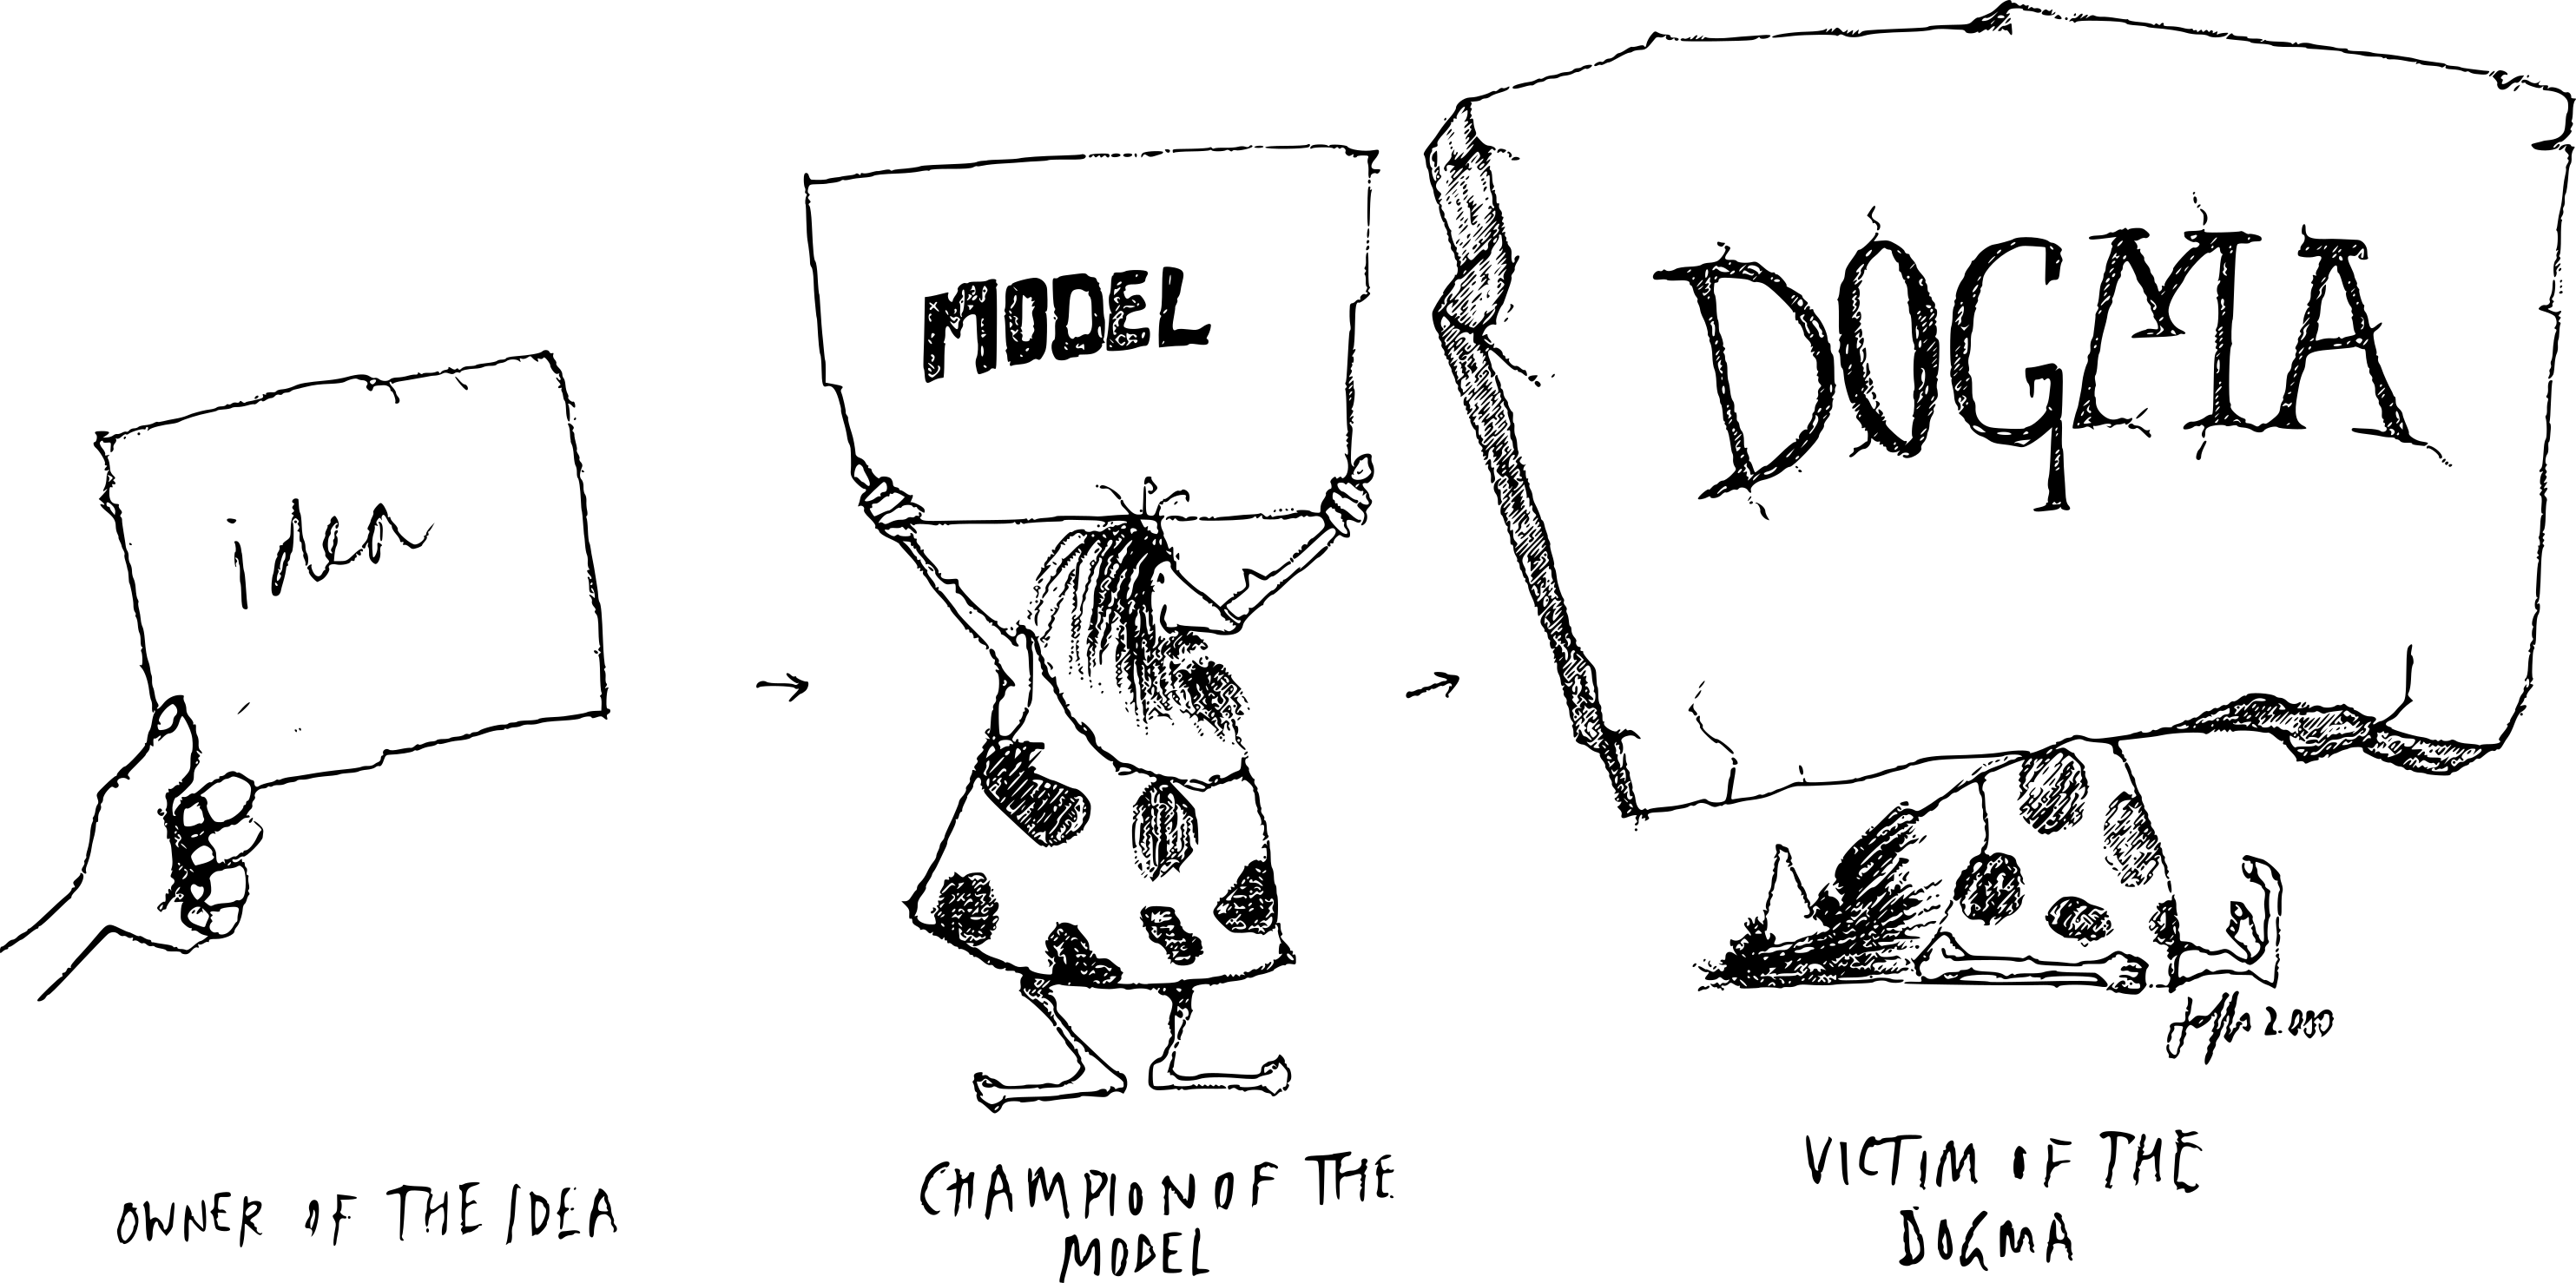
\includegraphics[width=\linewidth]{ch.discussion/imgs/dogma.png}
    \caption{\textbf{The phylotypic stage as a scientific dogma?} \cite{Caveman2000}.}
    \label{fig:dogma}
\end{figure}

There appears to be a concerning lack of genuine effort to understand or engage with one another's work within the field. Many studies, it seems, are riddled with glaring methodological issues that often go unaddressed, as long as they align with our prior beliefs. In chapters X AND Y I show and discuss a series of newly discovered problems with comparative approaches. I fear that highlighting these problems won't actually matter, as people will continue to believe their pet theories, and there will always be some methodology that in a way affirms it. For instance, during the early stages of my PhD, I had a meeting with one of the co-authors of the papers that applies transcriptomic comparisons between \textit{D. rerio} and \textit{X. tropicalis}\cite{marletaz2018}. He is a staunch believer of the hourglass model, and even has a tattoo of it! I shared some of my preliminary findings with him, which pointed to the inverse hourglass being an artifact of normalization. I also expressed my concerns regarding the methodology employed in their analysis. Surprisingly, he brushed off my concerns, stating that he was not directly involved in that particular analysis and thus saw no need to discuss its potential issues. Similarly, a colleague in my department once commented that despite my work showing that virtually all quantitative methodologies used in our field are flawed, the undeniable fact remains that the phylotypic stage does, in fact, exist.

Based on my own re-analyses, it appears most methodologies actually support the null model. The null model for evolutionary embryonic development would be that there is no specific stage of higher or lower temporal conservation. 
\begin{itemize}
    \item The hourglass-like pattern between zebrafish and frogs based on transcriptomic correlations can be explained by within-species correlations alone.
    \item The pattern of cell type proportion similarity between rabbits and mice, which is wrongfully called an hourglass, can be explained by discontinuous temporal sampling.
    \item Both the transcriptomic between-phyla inverse hourglass pattern and the morphological within-phylum inverse hourglass pattern are fully reproduced by simulated data with no specific temporal conservation.
    \item Only the \textit{Drosophila} enhancer conservation re-analysis results in a stage of maximum similarity, albeit at a different point than the original authors find. Moreover, I simply do not agree with the methodological approach of this analysis.
\end{itemize}
\noindent
Altogether, I have found little evidence to reject the null hypothesis of constant temporal conservation.

Furthermore, there is no consensus about what is actually expected to be conserved. The original observation that vertebrate embryos, perhaps, look more like each other at certain points in development than at other times, says nothing about the molecular basis for this. It has been quantitatively studied on the basis of embryonic lethality\cite{Uchida2018}, morphology\cite{OlafRP2003,Cordero2020}, DNA sequence conservation\cite{Piasecka2013,Quint2012,Liu2021} and activation order\cite{Uesaka2019}, cell type proportion\cite{Mayshar2023}, and whole-transcriptome similarity\cite{Piasecka2013,Irie2011,marletaz2018,Liu2020,Leong2021,PerezPosada2022,Kalinka2010}, with differing results. Measuring the transcriptome has become the most popular way to asses quantitative similarity. Is the widespread adoption of transcriptomic methods driven by a genuine expectation of transcriptomic similarity based on (supposed) morphological resemblance, or because transcriptomic methods are the most confirming of our prior beliefs that the phylotypic stage is the most conserved? Even assuming the phylotypic stage to exist, why would we expect to be able to measure such a complex phenomenon with such crude methods as observational studies and whole embryo sequencing?

Throughout the course of scientific history, certain theories, such as taxonomic phyla and the phylotypic stage, have evolved from initial concepts into widely accepted truths, creating a demand for a molecular explanation along the way. However, a fundamental issue arises from the loose and ambiguous definitions on which these theories are based, leading to their lack of predictive power and falsifiability, rendering them, by Popperian standards, non-scientific in nature. For instance, the concept of phyla hinges on the notion that animals sharing a common basic body plan are part of the same phylum, yet paradoxically, the basic body plan is defined as the morphological characteristics shared by all animals within the same phyla\cite{BUDD2000}. The definition of the phylotypic stage is similarly ambiguous. Historically, the pharyngula stage\cite{https://doi.org/10.1093/icb/21.2.391}, early somite embryo\cite{ https://doi.org/10.1046/j.1420-9101.1993.6030457.x}, and the tail bud stage \cite{Slack1993} have all been proposed as the vertebrate phylotypic stage. In quantitative studies, the choice of definition in turn depends on which stage exhibits the highest quantitative conservation. Consequently, the pharyngula \cite{Irie2011,marletaz2018}, the early somite embryo \cite{DomazetLoso2010}, or simply the stage(s) with the highest conservation metric\cite{Kalinka2010,Cordero2020} have all been identified as phylotypic stage. Our current approach to studying the phylotypic stage, where we selectively include definitions and ignore nonconforming studies, is not only wrong but also not useful.

\section{scepia: gene regulatory networks}

Almost all gene regulatory approaches are context specific. But in the end a single set of instructions (DNA) for all contexts.

\subsubsection{Move away from mRNA}

mRNA and protein relation.
The correlation between protein expression and mRNA expression seems high (0.87) measured across cell types. However, genes with high protein expression generally have high mRNA expression. So it is easy to get high prediction. If you want to predict a single gene you get correlation of 0.41. Simpson's paradox?!
https://www.nature.com/articles/nature23293

RNA-seq is used as a proxy for gene regulation, and simultaneously as a proxy for protein count/occurance. But transcripts are the measured effect of gene regulation. And transcipts correlate poorly.

https://www.biorxiv.org/content/10.1101/2023.05.23.541948v1

cool work of michael levine on xenobots

% https://twitter.com/nimwegenlab/status/1671923176626847744?s=12&t=oyB_faiBr8aHqHcjXZE50A

\begin{figure}[H]
    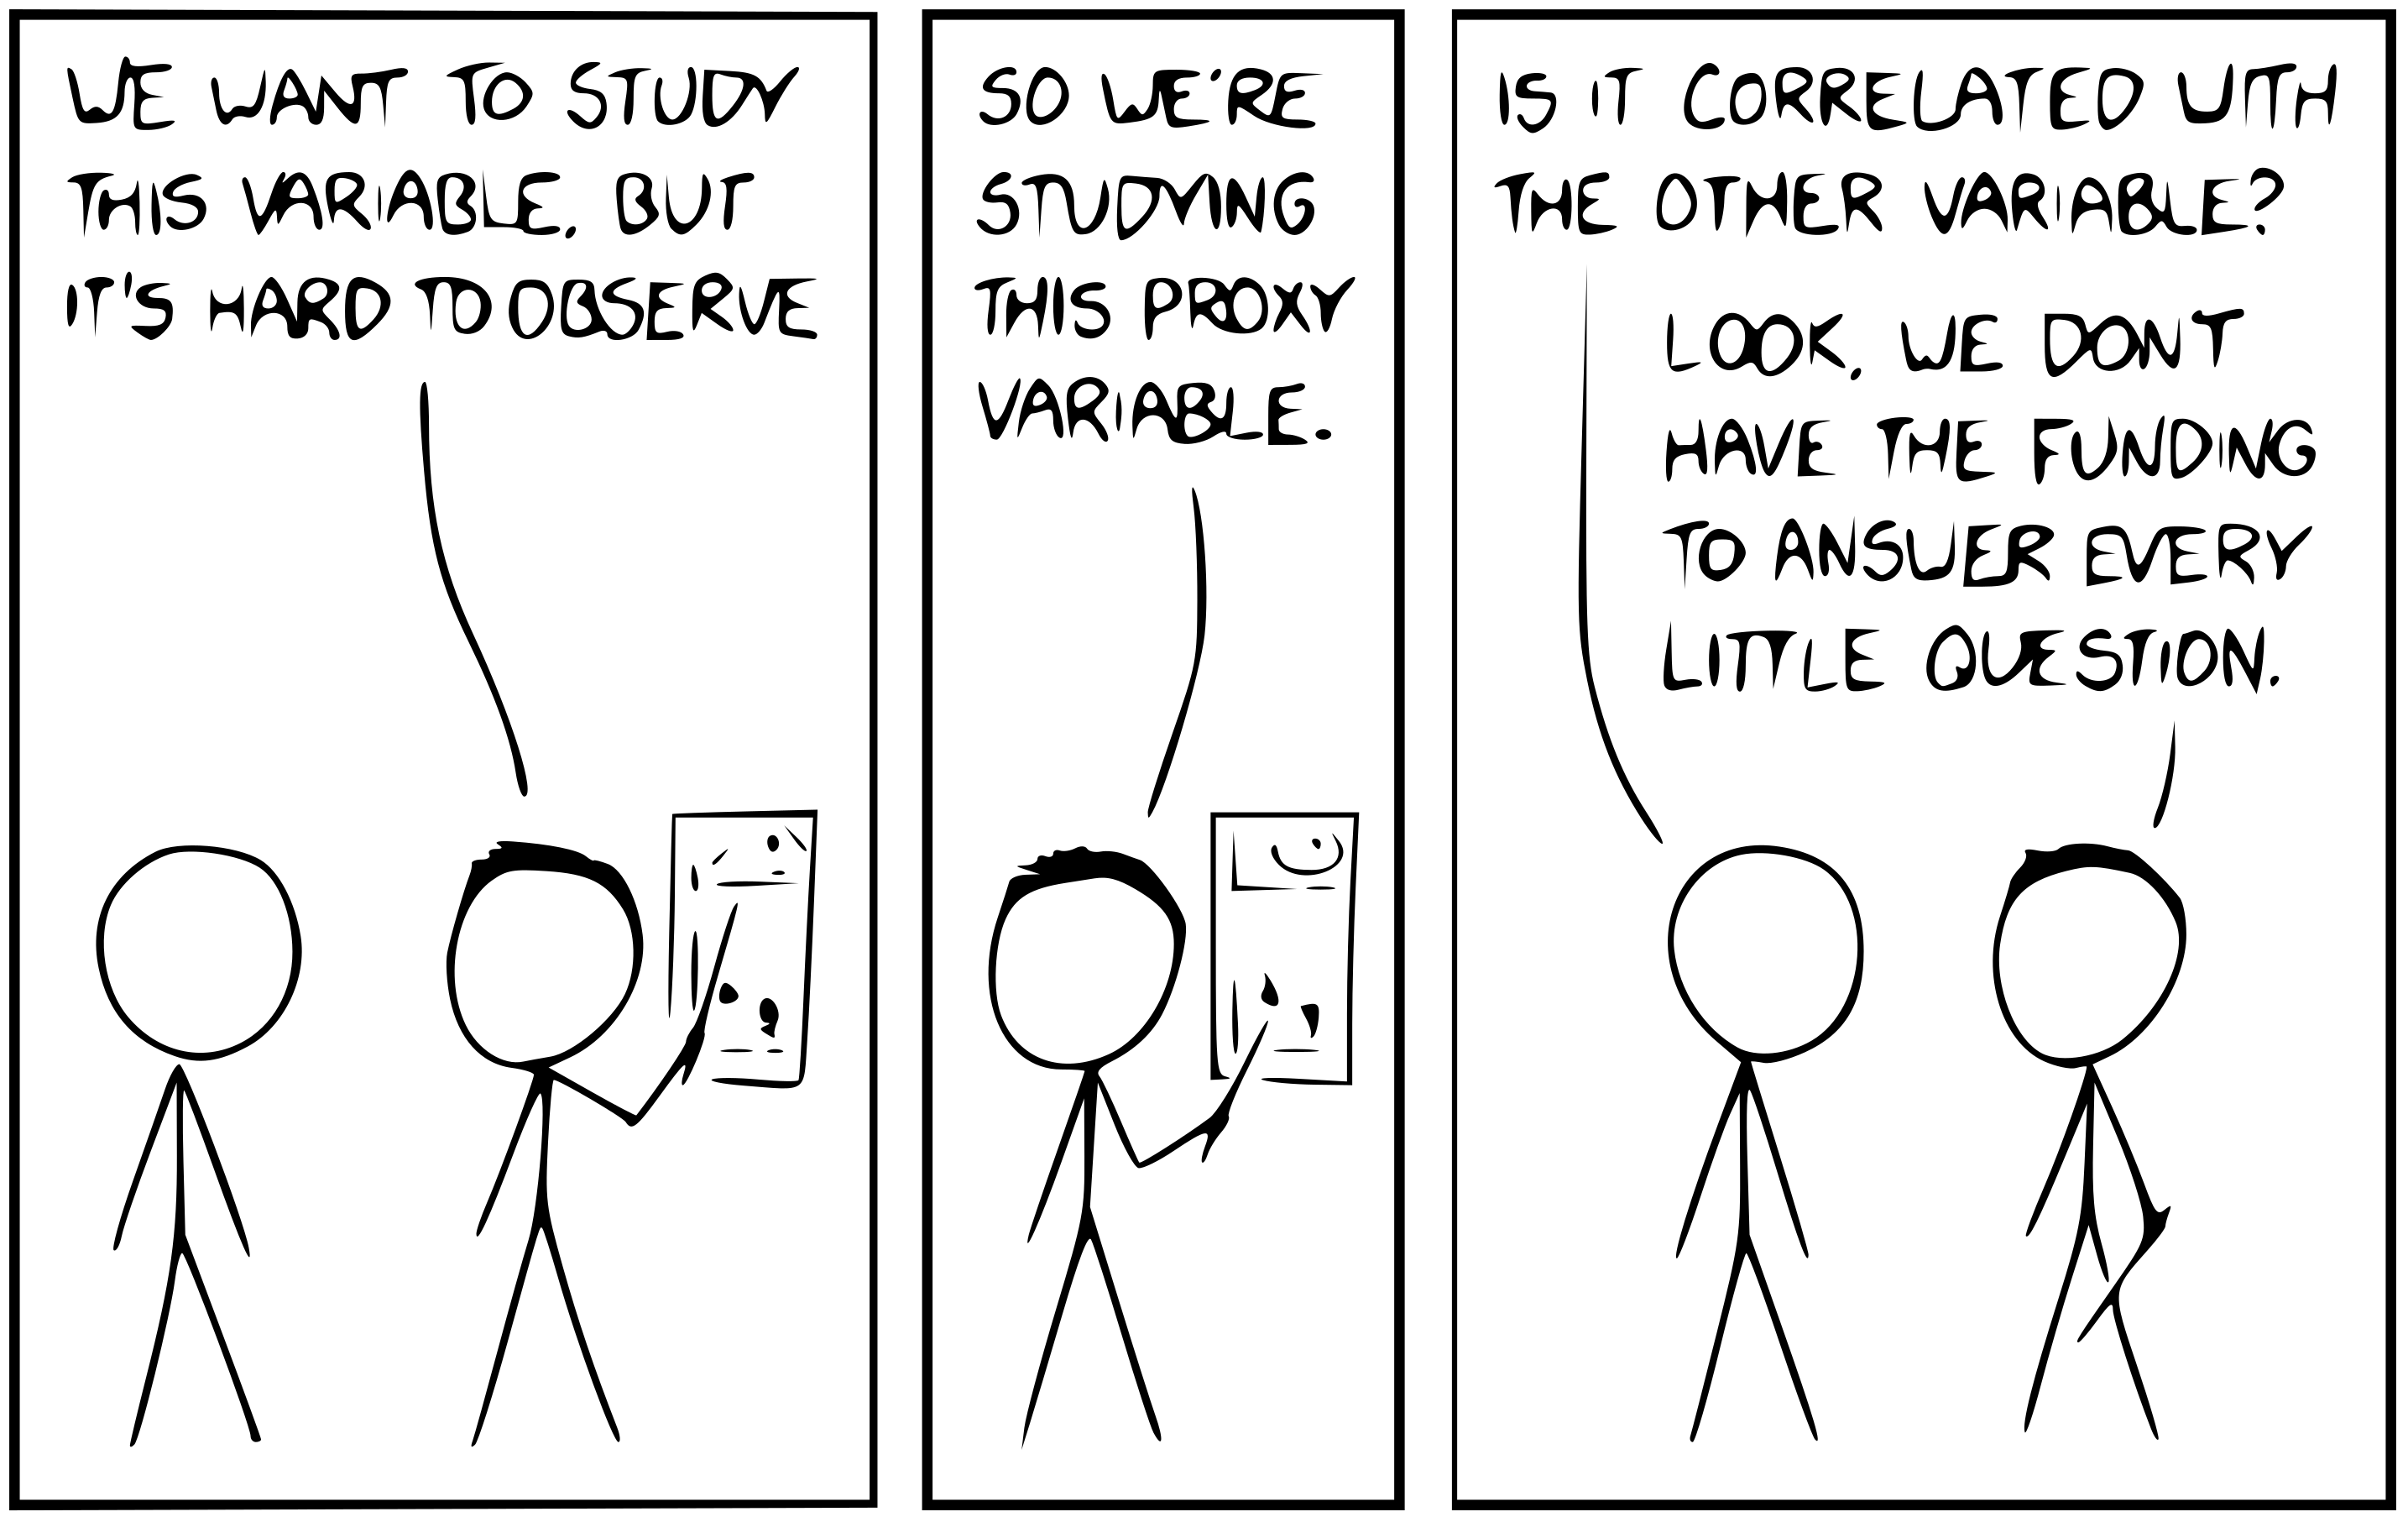
\includegraphics[width=\linewidth]{ch.discussion/imgs/xkcd.png}
    \caption{\textbf{RNA-seq is used as a proxy for gene regulation and protein expression}, but its relation to those is bad correlation TODO remains poorly understood. \textbf{xkcd}. URL: https://xkcd.com/2652}
    \label{fig:xkcd}
\end{figure}

\subsubsection{Universal gene regulatory networks}

\begin{enumerate}
    \item Comparison between two cases can not make predictions
    \item more data to train
    \item in the end single set of instructions (DNA)
\end{enumerate}

It doesn't make sense to make GRNs between two specific cell types, or two developmental stages. There is a single set of instructions (DNA). So it should be possible to have a single universal GRN. (e.g. avocado).

Moreover, perhaps it is important to ask ourselves what is ultimately the goal of these GRNs? Do we care about having a map with all the arrows? Because the current correlation-based networks won't help us with differentiation networks. 

\section{The growing burden of bioinformatics' technical debt}

\cite{Williams2019}

The scientific field of bioinformatics is a relatively young field and in a constant state of change, and thus regularly incorporates new technologies and insights. As such, doing a bioinformatics analysis is complicated, especially because biology is hard. Adding to this complexity is the use of outdated and poorly maintained software, and the development of inconsistent file formats and practices. These problems are exacerbated by the fact that a significant portion of bioinformaticians lacks formal training. In software development, this problem is known as "technical debt". Technical debt is analogous to financial debt, where you borrow money and must eventually pay it back, including interest. In the context of bioinformatics, technical debt represents outdated software and databases, and inconsistent file formats, and the "interest" is represented by the additional work required due to this debt. I am of the opinion that in the field of bioinformatics, the technical debt, has become so large that it has become prohibitive for analyses and new tool development. If the field does not address the issue of formally training bioinformaticians will progressively slow down.
% In the coming sections, I will highlight some of the problems I have encountered due to technical debt, and propose suggestions to reduce it.

Problem is getting larger?

Almost all sequencing data is shared on the Sequence Read Archive (SRA). The SRA is expected to contain 33 petabytes of data by the end of 2023, and is growing exponentially\cite{srawebsite,Katz2021}. It is an invaluable resource, and without it, my PhD research would not have been possible, as I have exclusively used public data. For scepia (chapter \textbf{TODO}) we had the idea to download all publicly available human h3k27ac data (12,000 samples) and use that as a reference database. A major problem in this analysis was that it is impossible to get automated sample annotation from the SRA, for instance, if a sample is from man/woman, the sample's age, tissue or celltype. This is mainly impossible because there is almost no information about samples on the database. Tools have been made to circumvent these issues, e.g. MetaSRA, ALE, and PredictMEE. These tools are imperfect, and should not even be necessary to begin with if the data is properly annotated. In the end, I simply decided to give up making this database, wasting time and computational resources. I can't find estimates of the cost of the SRA, but we can try. Currently, the SRA uses Amazon Web Services (AWS) for their data storage, which costs approximately 2 cents per gigabyte of storage\cite{amazon}, their 33 petabytes of data storage would cost approximately €660,000 per year. I am not sure to which degree EBI ENA and DDBJ mirror each other anymore, but if they fully mirror each other's sequencing data, just the cost of storage would between these three would be €2,000,000 per year. The 12,000 h3k27ac samples I downloaded consisted of 20TB of data, and downloading data from AWS costs approximately 5 cents per gigabyte\cite{amazon}.  We approximately used 300,000 CPU hours on Cartesius to process these samples, at 3 cents per CPU hour\cite{cartesius}, and 9 watts per CPU hour\cite{intelxeon}.
So my experiment roughly cost the SRA €1,000, Cartesius another €9,000, and almost one tonne of CO2\cite{CO2}. This could have been completely avoidable if the SRA had properly annotated metadata. Alternatively, a small-scale test on my side before starting this analysis would also have avoided these costs.

Not only is the SRA missing important metadata, but the sra-tools, a toolkit for downloading sequencing data, are also particularly difficult to use. When I started my PhD, these tools needed a complex start configuration before they could be used. This was particularly prohibitive for our seq2science fastq downloading implementation, as we couldn't expect our users to first run this configuration. Moreover, the conversion from the downloaded file to fastq took a long time and was not parallelized, even though the problem is easily parallelized. As a consequence others have resorted to making a parallel implementation (parallel-fastq-dump TODO CITATION). Downloading fastqs through the sra-tools is so bad that there are many tools that can be used to download fastqs so that the sra-tools don't need to be used: sra-explorer, pysradb\cite{pysradb}, fetchfastq, nf-core/fetchngs, and the seq2science download-fastq workflow. Similarly, the submission of new data is notoriously complicated, others are even making tools to streamline the process (https://bmcbioinformatics.biomedcentral.com/articles/10.1186/s12859-020-03694-0). Due to the complicated submission process, much data is probably incorrected added, for example drosophila dnase seq. Of the 20 samples, one was missing and two were swapped on the SRA. The SRA is a cool thing, saves lots of time by not having to redo experiments. But at the same time its poor implementation makes it so that more work.

% TODO where to put this?
% A well-known example of how the lack of computational skills affects bioinformatics is 
% Excel gene names?
% % British government used EXCEL to store their covid results. When they reached maximum rows they couldn't add more.
% https://oct4th.sandbox.bio/
% http://maplab.imppc.org/truke/
% Gene Updater
% Beta'cop gene name
% Conversion between transcript ids and gene ids is a pain. Especially between different databases. Third party mygene.info is real life saver.

% Ensembl genomes just disappearing! BDGP6.32
% They use a mixture of Ensembl version and assembly versions. Weird

The most common file formats in bioinformatics have been designed in the 90s and 00s, and as such reflect the tools of their time. Most file formats are text-based and human-readable, where each line represents a feature, for instance, a sequencing read. This design made sense at its time, as awk and perl were popular programming languages. Even though this design might not always be the most performant, it has a clear advantage where one can scroll through the files and easily search for certain features. What however is not clear to me, is the strange inconsistencies among these formats. For example, the sam, bam, bed, gtf, and vcf file formats all specify features and their position in the genome. A coordinate system can be either zero- or one-indexed , and whilst zero-indexed makes the most sense, as long as all formats make use of the same coordinate system it is easy working between them. However, the bam and bed format are zero-indexed\cite{Li2009}, whilst the sam-, gff, and vcf-format are one-indexed\cite{Li2009,Danecek2011}. This means that it is extremely easy to make one-off errors when looking for overlapping features between these formats. This incurs significant development time for anyone working with these files, and more importantly, increases the odds of making mistakes. 
https://www.cs.utexas.edu/users/EWD/transcriptions/EWD08xx/EWD831.html

% Similarly 
% Fastq format is okay. 
% Made by industry.
% Who thought it was a good idea to split fastq files? 
% Which data format ever splits over multiple files?
% From a single fastq, to paired-end. Annoying, but fine. But now single-cell sequencing adds another file, the barcode and umi. 
% Single cell datasets often useless as only two out of three reads submitted.
% Single cell also suchs because barcodes are often not submitted to SRA.
% https://support.10xgenomics.com/single-cell-multiome-atac-gex/software/pipelines/latest/using/fastq-input
% R1, R2, and R3?!
% Implementing 

The fasta format is for genomic sequences. The file format works fine, and was developed in 1985 (https://www.science.org/doi/10.1126/science.2983426). The problem with the fasta format is that there are natural differences between individuals, and as such there is a certain level of variety of DNA sequences. This is particularly important for medical stuff, hence projects as the million genomes project. The variety can be single nucleotides polymorphisms, which the fasta format can handle to some degree by e.g. ambiguity characters such as N. But longer stretches of alternative sequences the fasta format can not deal with. Since human genome assembly number 38 (hg38/grch38) that was released in 2013, alternative stretches of sequences have been added to the fasta. This means that for certain of the DNA multiple sequences are added to the fasta. A major improvement, especially in the case of medicine and non-western individuals, as the original human genome assemblies were mainly based on western. However, the common approach to dealing with the alternative regions in hg38 is to just remove them and ignore that they exist. Even more surprising is the lack of usage of the hg38 assembly, with the previous genome assembly hg19 being seemingly more popular. A quick and dirty check on \url{https://app.dimensions.ai} shows that there are currently 9,579 publications mentioning hg19 vs. 8,796 publications mentioning grch38. People prefer to use hg19 from 2009, instead of the more complete hg38 genome. No one is going to use T2T genome. Million genomes project is a pipe dream, as alt regions exist for ten years but it is mostly ignored.

% Many many times I have come across a .Rds file. WHAT!
% Also people can just make up their own format. Depends on popularity of group (or format?) on adoption. D4 dataformat. Bustools. 
% genrich, really nice. Outputs bedgraph-ish values... 

MACS(2) by far the most popular peak caller. MACS2 should get credit for its continuous development. Nevertheless, MACS2 is particularly idiosyncratic with ATAC-seq peak-calling. With ATAC-seq peak-calling one is interested in the cleave sites, which means the beginning and end of the template. Tao Liu, one of the main developers of MACS2, recommend to run the algorithm in paired-end mode. (https://github.com/macs3-project/MACS/issues/331) This means that MACS2 makes a pile-up between the start and end of the template. This is not what we are interested in. Ideally one would take the region around the start and end of the template. By using the shift and extend options in MACS2 one does this, but somehow then all the mates are discarded leaving us with half the data. To properly do ATAC-seq peak calling one then has to make a script that convert a paired-end BAM to single-end, and then shift extend works....? Similarly, since its implementation in 2008, MACS2 did not support more than two replicates, however multiple replicates is a good thing. When more than two replicates were used, researchers used to pool the replicates together and called peaks on them as if no replicates were used. How come I, as a first year PhD student, had to implement this for MACS2 more than ten years after its initial release (\url{https://github.com/macs3-project/MACS/pull/304})?
% I can't make the case that better peak callers exist because benchmarking is hard, but there are more performant and better documented onces. For instance genrich, re-implementation of macs2 which is more performant, better defaults, and different assumption\cite{genrich}.

The quickest developing part of molecular analyses currently is the field of single cell analyses. As a consequence, the most shortcuts are taken in these analyses. A partical painful shortcut is the difference in log fold change between Seurat and Scanpy. Seurat and Scanpy are X, for Python and R respectively. The scanpy implementation calculates the mean of the log changes, whilst the Seurat implementation calculates the log of the means. The implementation of Seurat is sensitive to outliers, and should be changed. This difference results in wildly different outputs between these two tools, even though they claim to do the same. The bug has been reported more than 10 months ago, and so far was fixed incorrectly https://github.com/satijalab/seurat/issues/6654. Double dipping
Statistical tests over cells, not good. 
Reporting p-values that are nonsensible.
Refer to pubpeer?

Apart from trimming and alignment, most algorithms are usually implemented extremely poorly. Take a look at my \textit{bad} quantile normalization implementation in Python. It really should not use that much memory, and it probably could easily be 10-100 times faster in a different language. The solution to these problems is to make the software better, however the usual solution in the field is to make the hardware better. Increasing the hardware capacities makes it look like what you are doing is smort. Our department has a server with 503 GB of RAM. This was frequently not enough to run ANANSE, a tool developed by our department. The solution wasn't to make ananse more memory efficient, but (a bit oversimplified) we just bought a new server with double the RAM. Apparantly an ex colleague even specifically requested a computer with 4,000 GB of RAM so he could run his analyses. 
Something about running time? green algorithms? 

To avoid that this is unconstructive rant:

Biological analyses are extremely complex. 

Something positive about progress, lots of interesting discoveries! 
Some conclusion, about that this is a limiting factor. Field is new and always moving. But its pretty bad. No proper education. Supervisors are not able to train their students in these analyses. Someone that did PhD 20 years ago worked with microarray, ten years later, when they become group leader, 
Feels to me that bioinformatics is at a crossroads, start putting emphasis on high quality code/databases/... or be stuck at a low level of efficiency as a field. Wasting resources, time, and opportunities.
Funding not aligned!
Why the heck did we publish seq2science? No maintainers... Waste


% phylotypic stage analyses are bad :). Doing a quick and dirty analysis is okay. But somehow, my re-analysis had to be extremely thorough. Not only do I have to re-do their analysis, I have to pay the interest of their sloppy work. In chapter SCEPIA TODO I also take lots of quick and dirty stuff... :(

% \subsection{Too much descriptive, not enough understanding}

% Early adopters have been overwhelmed by the size of the data, lack of analytical tools, but mostly the number of different cell types generating a flurry of research articles with titles like "single cell sequencing in tissue X reveals heterogeneity".  

% % \subsection{Stop blaming "the incentives"}

% % incentives: https://www.talyarkoni.org/blog/2018/10/02/no-its-not-the-incentives-its-you/

% % \section{Do I regret seq2science?}


% \subsection{Self-correcting}

% e.g. wild growth covid papers

% papers keep on being cited after retraction or criticism. Number one paper of percentage of genome is functional gives highly criticized ENCODE paper. ENCODE claiming 80\% biochemical and criticism on it. When googling first result is ENCODE (I think)

% Our golden standard is actual clinical trials! Our methods don't seem to work so well..?
% https://www.ncbi.nlm.nih.gov/pmc/articles/PMC6409418/
% https://journals.plos.org/plosmedicine/article?id=10.1371/journal.pmed.0020124

% % Biology is messy, but that does not mean computational biology has to be.
